\documentclass[12pt,a4paper]{report}
\usepackage[onehalfspacing]{setspace}
\usepackage[a4paper, total={6in, 10in}]{geometry}
\usepackage[utf8]{inputenc}
\usepackage{graphicx}
\usepackage{wrapfig}
\usepackage{booktabs}
\usepackage{amsmath}
\usepackage{hyperref}
\usepackage{float}
\usepackage{pgfplots}
\usepackage{subcaption}
\graphicspath{{img}}
\usepackage{algorithm} 
\usepackage{algpseudocode} 
\usepackage{amsmath,amsfonts}
\usepackage{listings}
\usepackage{xcolor}
\usepackage{listings}
\usepackage{xparse}
\usepackage{soul}
\usepackage{minted}
\usepackage{etoolbox}
\patchcmd{\thebibliography}{\chapter*}{\section*}{}{}

%%%%%% Bibliography %%%%%%
% Replace "sample" in the \addbibresource line below with the name of your .bib file.
\usepackage[style=ieee, 
citestyle=numeric-comp,
sorting=none]{biblatex}


\addbibresource{test.bib}

\title{K-Nearest Neighbors(KNN)}
\author{Yohannis Kifle Telila}
\date{October 2021}

\pgfplotsset{compat=1.18}
\begin{document}
\begin{titlepage}
\begin{figure}[t]
    \centering
\includegraphics[width=0.4\textwidth]{images/cherubino.eps}
\end{figure}

\begin{center}
    \textbf{University of Pisa\\Graduate Programme in Computer Science}
    \vspace{15mm}
    \\
    {\huge{K-Nearest Neighbors(KNN)}}\\
    \vspace{5mm}
    \large{Yohannis Kifle Telila} \\
    \vspace{2mm}
    \large{Student ID : \textbf{621821} }
\end{center}

\vspace{20mm}
\begin{center}
    {\large Parallel and distributed systems: paradigms and models\\Academic year 2021/2022}
\end{center}
\vspace{36mm}
\end{titlepage}

\tableofcontents
\pagebreak

\chapter{Introduction}
\section{Problem description}
In this project I will be analysing and comparing performance of  different implementations of K-Nearest neighbours algorithm. The problem statement is provided as "given a file containing 2D points separated by comma, one point per line the problem is to find K Nearest points for every points in the file". The distance is measured using euclidean distance measurement. Point $i$ is the point whose coordinates are listed in line $i$ on the file. The output is a set of lines each hosting a point id and a list of point ids representing its KNN set ordered with respect to distance. \\ 

The problem of finding a K-nearest neighbour of a given points can be parallelized to speed up the computation. We can categorize this problem as \textbf{data parallel computation} or \textbf{embarrassingly parallel computation} because its possible to divide our computation to a number of workers and combine the result at the end and communication between the threads(workers) is not needed. \\

In this report, I will be discussing the results I get from three different implementation of the problem and improvements on the original implementation to get better performance of the problem. The first method I used to implement is pure STL C++ in sequential method. This implementation is provided in the file \textbf{stl\_seq\_knn.cpp}. Secondly, I used the same implementation and parallelized it to speedup the computation using multiple threads. The implementation of this version can be found in \textbf{stl\_par\_knn.cpp}. Thirdly, I used openMP \verb!parallel for! to implement the same problem in a parallel form. The code for this implementation can also be found in the file \verb!openmp_par_knn.cpp!. Finally, I used FastFlow parallel for reduce version where the implementation can be found \verb!ff_pf_knn.cpp! in the file provided along with this report file.

\section{Algorithm}
As stated in the problem statement, we are interested in finding the $k$-nearest neighbours for each given points in 2D space. To find k-nearest neighbour of a point, the first solution would be to sort all the points based on the distance, from nearest to the furthest and selecting the top $k$ nearest points which will be our K-nearest neighbours for that point. But this would require to store all the points which might not be efficient in case we have huge amount of points. The best solution would be to store only the result in priority queue of size k and continuously update our k points and discard other points. The pseudo code for sequential implementation is provided below.

\begin{algorithm}
	\caption{K-nearest neighbour} 
	\begin{algorithmic}[1]
	    \State $points2D \gets $read2Dpoints(filename)
	    \State $vector<knn\_res> \hspace{0.3cm} $knn\_imp\_result    
		\For {$i=0,1,2,\ldots,points2D.size()-1$}
			\State $knn_{i} \gets $get\_knn(points2D, points2D.size(), i,k)
			\State ${\_} $Insert(knn\_imp\_result,knn\_{i})
		\EndFor
	\State print(knn\_imp\_result)
	\end{algorithmic}
	\label{knn:alg}
\end{algorithm}

\verb!knn_res! is a user-defined data structure containing \verb!int index! to store index of the point and \verb!vector<int> knn_index! to store index of all the nearest points. The method \verb!get_knn(points2D,points2D.size(), i, k)! will receive the 2D points read from the file, the size of the 2D points, point index \textbf{\textit{i}} and number of nearest neighbours \textbf{\textit{k}} and returns a vector containing \textbf{\textit{k}} nearest points for the point \textbf{\textit{i}} . The pseudo code for this method provided at Algorithm \ref{getknn}.

\begin{algorithm}
	\caption{get\_knn method pseudo-code} 
	\begin{algorithmic}[1]
	    \For {$j=0,1,2,\ldots,points2D.size()-1$}
			\If{$J$ not equal \textit{i}}
                \State $d \gets $measure\_euclidean\_distance(points2D[i], points2D[j])
                \If{$kneighbours\_size$ $<$ \textit{k}}
                    \State ${\_} $Insert(kneighbours,d,j)
                \EndIf
            \If{$kneighbours\_top\_distance$ $>$ \textit{d}}
                \State ${\_} $kneighbours.remove\_from\_top()
                \State ${\_} $Insert(kneighbours,d,j)
            \EndIf
            \EndIf
		\EndFor
	\For {$i=0,1,2,\ldots,k-1$}
	        \State ${\_} $Insert(knn\_res\_i,kneighbours.top().index)
	        \State ${}$\_remove\_from\_top\_kneighbours.
	\EndFor
	\State ${return} \hspace{0.3cm} ${knn\_res\_i}
	\end{algorithmic}
	\label{getknn}
\end{algorithm}

The completion time or $T_c$ of this algorithm can be estimated as the sum of time it take to read the points from a file $T_{read}$, the time it takes to compute the nearest neighbours of the points $T_{compute}$ and the time it takes to print the result to a file $T_{write}$.

\begin{equation}
T_c = T_{read} + T_{compute} + T_{write}
\end{equation}

The time $T_{compute}$ is the largest of all three time measures which could be reduced significantly by farming the computation to multiple workers. The time $T_{read}$ and $T_{write}$ are done sequentially and can't be parallelized. These two time measures are accountable for sequential fraction of our code. But for parallel version of our code the sequential fraction of our code would also include the time it take to divide the task to the threads(workers) $T_{divide}$ and $T_{collect}$. If we managed to make small change in our implementation it could be possible to remove the time it takes for partial results collection $T_{collect}$. So the $T_c$ for parallel version is given as. 

\begin{equation}
T_c = T_{read} + T_{divide} +  T_{compute} + T_{write}
\end{equation}

The sequential fraction for parallel version would be the sum of $T_{read}$, $T_{divide}$ and $T_{write}$. The parallel fraction would be $T_{compute}$.

\begin{table}[htp]
  \begin{center}
    \begin{tabular}{l c c} % <-- Alignments: 1st column left, 2nd middle and 3rd right, with vertical lines in between
      Test Data & $T_{read}$ (sec) & $T_{write}$ (sec)  \\
      \midrule
      input\_20k\_s123.txt  & 0.157 & 53.364 \\
      input\_50k\_s456.txt  & 0.373 & 262.247 \\
      input\_100k\_s789.txt & 0.737 & 1125.713 \\
      \bottomrule
    \end{tabular}
    \caption{Read and write time for $k=50$}
    \label{readwritetime}
  \end{center}
\end{table}

For the sake of the experiment, I excluded the $T_{read}$ and $T_{write}$ for each experiments which can be achieved by placing $-d$ flag during execution. Detail will be provided in the last chapter.

\chapter{Parallel Implementation choices}
In this section, I will discuss different parallel implementation choices I experimented with.
\section{C++ STL Parallel}
My first implementation was to parallelize the for loop computation on line 3 of Algorithm \ref{knn:alg} using threads. There is the second for loop inside \verb!get_knn()! method on algorithm \ref{getknn} which could also be parallelized. If we were to parallelize this for loop we need to synchronize the workers which creates an additional overhead. Depending on the available resources, we could potentially get a better performance parallelizing both the outer and inner for loops. For this experiment I only parallelized the outer for loop and the inner for loop is performed sequentially by each workers. \\

The amount of task between the workers is distributed in a static partition schema. I divided the data-set into equal size of chunks based on the number of workers and the first worker gets the first chunk, the second worker will get the second chunk and so on. This way all the workers will get fairly equal amount of work. The work load of the workers is also fairly balanced since each workers get same amount of data. Ideally, the time it takes to compute the $k$-nearest neighbours of any point should be equal. \\

Each workers writes their partial results \verb!par_res_chunk! of the knn computation to the global result \verb!knn_par_result!. Since many workers could try to access the global result at the same time, I used \verb!std::mutex! to synchronize access to this global variable \verb!knn_par_result!. The C++ STL implementation can be visualized as figure \ref{fig:stl_par} \\

\begin{figure}[H]
    \centering
    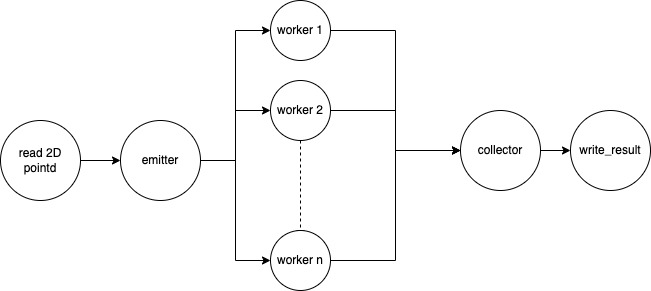
\includegraphics[width=\textwidth]{images/stl_par.jpg}
    \caption{C++ STL implementation}
    \label{fig:stl_par}
\end{figure}

The code implementation is found under the name \verb!stl_par_knn.cpp! and the parameter to this implementation are the number of workers, the value of \verb!k!, input file data containing the 2D points and optional flag \verb!-d!.

\section{FastFlow}
I used a \verb!ff::parallel_reduce! method which provides easy interface to map operation over the number of workers and do the reduction easily for iteration in-dependant operations. I used static partitioning, which will finally produce ordered output.
\section{OpenMp}
For the openMp version I used \verb!#pragma omp parallel for!, which spawns a number of threads where each threads executes a chunk of of the entire for loop. I used the static scheduling for the task distribution among the workers. Diagram for this implementation can also be visualized as in \ref{fig:stl_par}. Synchronization of the thread is performed using \verb!#pragma omp critical! where the partial result computed by the threads is merged with the global result.
\chapter{Experiment setup and performance measurements}

To test the performance of my implementations, I used a remote machine with processor \textbf{\textit{Intel Xeon PHI 64-cores } with 4 way hyper-threading}. Each core has the speed of 1.30GHz. In every experiment I excluded the time for for reading the file and writing the results. But the time for dividing task and collecting the partial results from the workers in parallel implementations is included in the time measurement. The read and write time is provided in table \ref{readwritetime} \\

The test was  performed on \textit{\textbf{nw}} $\in$ \textbf{\textit{\{1,2,4,8,16,32,64,128,256\}}} and all execution time was measured using \verb!utimer.cpp! class which uses RAII (Resource acquisition is initialization) for measuring time. the experiments were performed with \textbf{\textit{k}=50} and the time was averaged over three runs.
\section{Data-set}
As the input for the algorithm and to test the performance of the algorithm, I generate three different size of 2D points files. Namely, \verb!input_20k_s123.txt!, \verb!input_50k_s456.txt! and \verb!input_100k_s789.txt! which all can be found inside \verb!/data! folder.
\begin{table}[htp]
  \begin{center}
    \begin{tabular}{l c c c} % <-- Alignments: 1st column left, 2nd middle and 3rd right, with vertical lines in between
      Test Data & Size & Range & Seed  \\
      \midrule
      input\_20k\_s123.txt  & 20,000 & (-100,100) & 123 \\
      input\_50k\_s456.txt  & 50,000 & (-100,100) & 456 \\
      input\_100k\_s789.txt & 100,000 & (-100,100) & 789 \\
      \bottomrule
    \end{tabular}
    \caption{Dataset used for experiment}
    \label{readwritetime}
  \end{center}
\end{table}

These three data-set would help us understand how our algorithm would behave in smaller, medium and bigger data sets. The code used for the data-set generation can be found at \verb!generate2d.cpp!.  Guide on how to run this code is provided in the last chapter.

\section{Speed up($S_p$)}
The speed up of a parallel algorithm is given as the ratio of best execution time in sequential algorithm over to the time for parallel algorithm. Mathematically speed-up can be expressed as.

\begin{equation}
S_p(nw) = \frac{T_{seq}}{T_{par}(nw)} 
\end{equation}

The speedup indicates the improvement in performance from adding more processing units to the system. Ideally, we would expect the speed-up to be equal to the number of workers(threads) but this is usually will never be quite achieved because of the overhead that will be introduced as we add more processing units to the system.

\section{Scalability($S_c$)}
Scalability of a parallel program with $nw$ workers can be expressed as the ratio between time spent using only one processing unit over time spent using $nw$ workers. This can be expressed mathematically as.

\begin{equation}
S_c(nw) = \frac{T_{par}(1)}{T_{par}(nw)} 
\end{equation}

The value we would get from calculating scalability will tell us how much we can improve when we add more computing resources. Again, ideally we would expect a linear increase in scalability as we add more workers to our system but its impossible to achieve this result because of the overhead that will be introduced.

\section{Efficiency($E_f$)}
The Efficiency of a parallel program is the ratio of speed-up we obtained over number of workers or processors used which can be expressed as.

\begin{equation}
E_f(nw) = \frac{Sp_{nw}}{nw} 
\end{equation}
The max value for $E_f(nw)$ is 1.

\chapter{Results}
In this chapter I will be discussing the results found by running the implementation choices described under chapter 2. Only the plots for the  \verb!input_100k_s789.txt! data-set will be provided in this section. The plot for the rest of the data set will be provided at the end of this report page.
\section{Sequential implementation}
The sequential implementation is the one provided in algorithm \ref{knn:alg}. The  code for this implementation can be found at \verb!stl_seq_knn.cpp!. The table \ref{seqresulttable} summarizes result I achieved over the three data sets.

\begin{table}[htp]
  \begin{center}
    \begin{tabular}{l c c c} % <-- Alignments: 1st column left, 2nd middle and 3rd right, with vertical lines in between
      Threads & Test Data & Time(sec)  \\
      \midrule
      1 & input\_20k\_s123.txt  & 14.7877 \\
      1 & input\_50k\_s456.txt  & 90.069 \\
      1 & input\_100k\_s789.txt & 349.335 \\
      \bottomrule
    \end{tabular}
    \caption{STL C++ Sequential result}
    \label{seqresulttable}
  \end{center}
\end{table}
This result will be used to measure the speed up of the parallel implementations.

\section{Speed-up comparison}
From the speed-up graph of the three implementation choices depicted in Figure \ref{speedup-main} we can understand that the FastFlow version of the parallel program achieved a better performance compared to the other two as the number workers grows.
\begin{figure}[H]
    \centering
    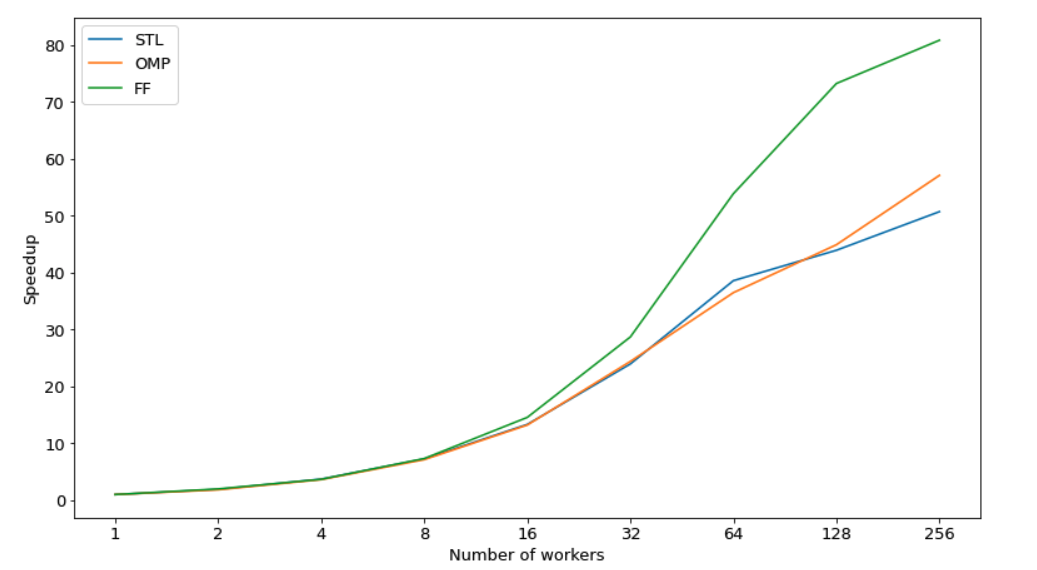
\includegraphics[width=\textwidth]{images/main-speedup.png}
    \caption{input\_100k\_s789, Speed-up plot, K=50}
    \label{speedup-main}
\end{figure}
 From the plot, we can observe that all three methods followed the ideal speed-up until the number of workers reaches \textbf{32}. While the FastFlow version showed even a more closer speed-up value to the ideal speed-up until the number of workers reach around 50, the other methods diverged and plateaued from ideal speed-up. This is mainly caused by the overhead and bottlenecks that comes with the increase in the number of workers. In the next chapter, I will discuss more in detail possible improvements on openMp and STL Cpp version to increase speed up. 
\section{Scalability comparison}
The same observation as in the speed-up can be seen in the scalability plot. We would expect an increase in scalability as the number of workers gets bigger. 
\begin{figure}[H]
    \centering
    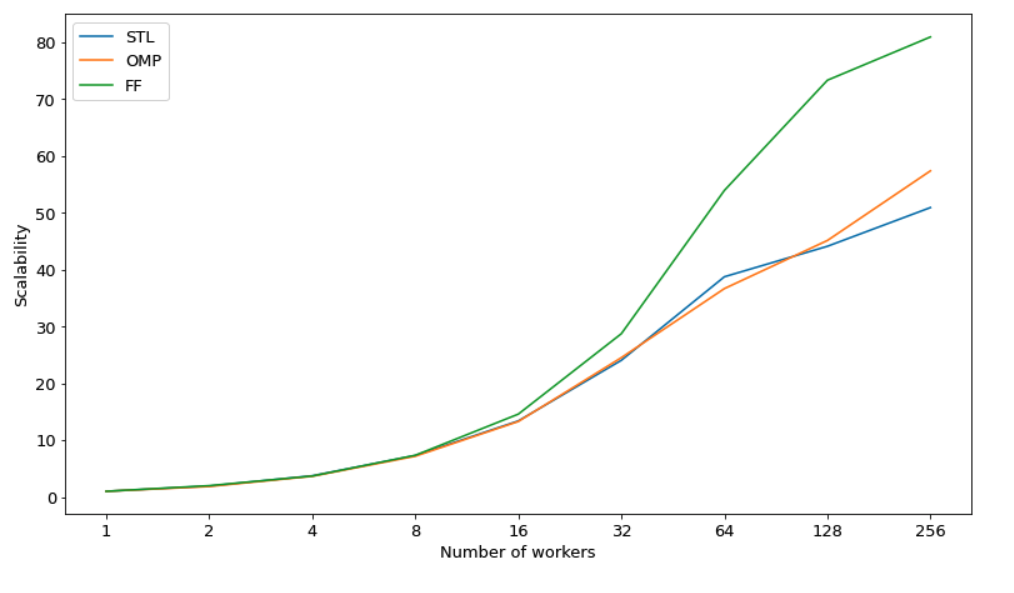
\includegraphics[width=12cm]{images/main-scalability.png}
    \caption{input\_100k\_s789, Scalability, K=50}
    \label{scalability-main}
\end{figure}
 
 As we have discussed in chapter 3, it could difficult to get to the ideal scalability which we can observe from the plot. As the number of workers increase, the scalability becomes more and more less than the ideal value. \\
 
 Interestingly, as we would expect, as the amount of data-set gets bigger, the overheads will be become more and more negligible. We can observe this from the result of the three data-set. With data-set containing 20,00 points, the overhead starts to make an effect starting from around nw = 8. Whereas, with the data-set 50,00 points, the effect of the overhead stops being negligible starting from nw=32. For the data-set with 100,000 points, the critical points is around nw=50. This is what is stated in the Gustafson's law.
\section{Efficiency comparison}
Here again the efficiency quickly drop for the two implementation openMp and STL C++ after 8 number of workers where as the efficiency was between 1 and 0.8 until the number of workers reaches 70 for the FastFlow version.
\begin{figure}[H]
    \centering
    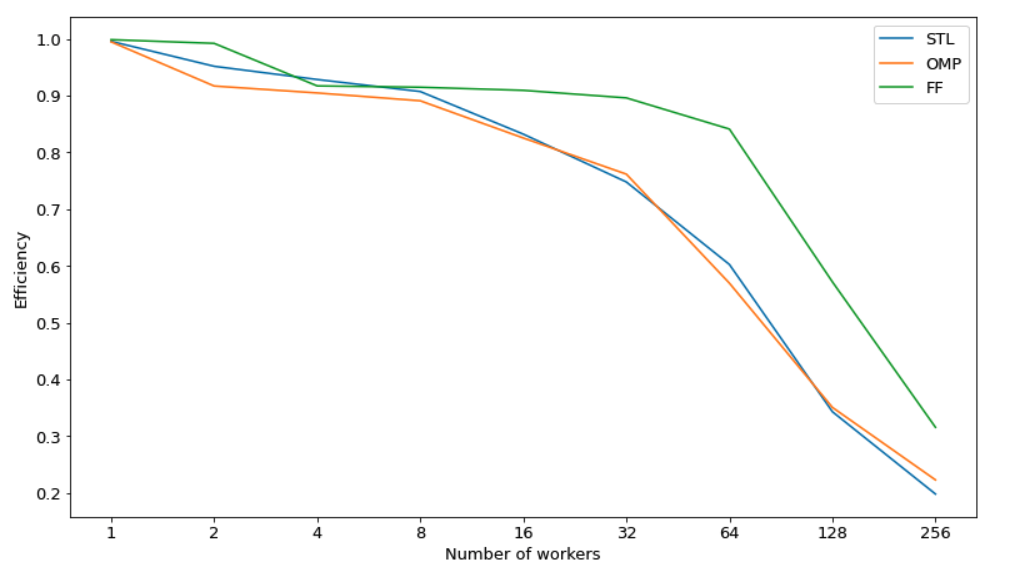
\includegraphics[width=\textwidth]{images/main-efficiency.png}
    \caption{input\_100k\_s789, Efficiency, K=50}
    \label{scalability-main}
\end{figure}

\chapter{Performance improvement}
From the previous result chapter, it is clear that the two implementation choices, STL CPP and openMp didn't quite show a good performance. The obvious one reason is the bottleneck, where each thread writes their partial result to the global result. Let's see this improvement in detail and the result I was able to get.
\section{Removing bottleneck}
One way to avoid this bottleneck is to create a vector of size equal to the number of workers and passing the address of the index to the corresponding thread. This way, each thread will be able to write their results to the global result without the need of exclusive access to the global result. The updated implementation of parallel STL C++ can be found at \verb!stl_par_knn_nobottleneck.cpp! and for openMp the code can be found at \verb!openmp_par_knn_nobottleneck.cpp!.
\section{Pinning thread}
The other potential event that could cause additional overhead is the movement of threads from one core to another. During the execution the threads may be subjected movements to another core and this is totally handled by the operating system. When a thread is moved to another core, all the data that is stored in a cache will also be moved to the new core which will cause an overhead. The solution to this event is to pin the threads to a core during their entire execution period. Thus, saving the time it take to move one threads from one core to another.
\section{Updated Result}
I re-run the test with the updated version of the implementations and I was able to almost match the performance I was able to get using FastFlow. Again, I will only be showing the results I managed to get using the data-set \verb!input_100k_s789.txt! here.

\begin{figure}
     \centering
     \begin{subfigure}[b]{0.45\textwidth}
         \centering
         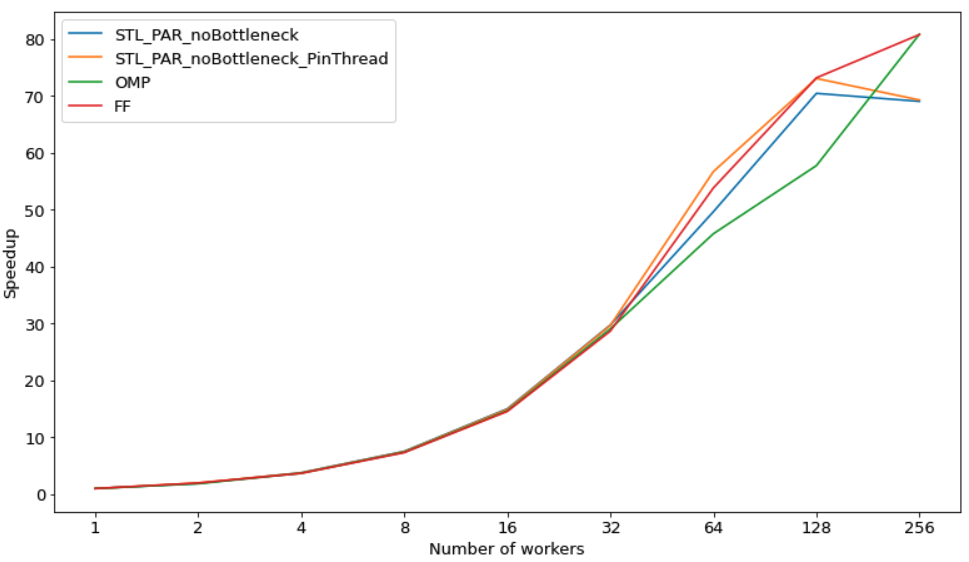
\includegraphics[width=\textwidth]{images/optimized-speedup.png}
         \caption{Speed up}
         \label{fig:y equals x}
     \end{subfigure}
     \hfill
     \begin{subfigure}[b]{0.45\textwidth}
         \centering
         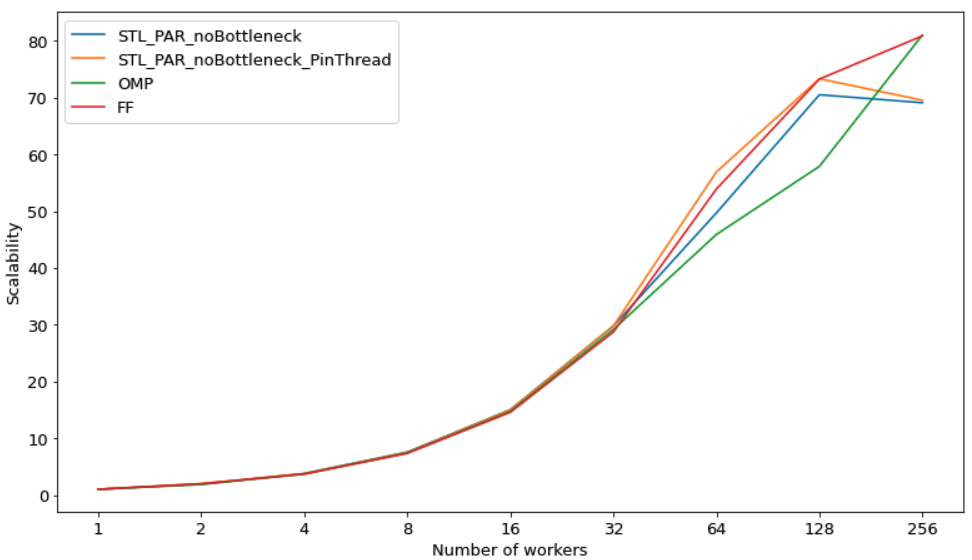
\includegraphics[width=\textwidth]{images/optimized-scalability.png}
         \caption{Scalability}
         \label{fig:three sin x}
     \end{subfigure}
     \hfill
     \begin{subfigure}[b]{0.45\textwidth}
         \centering
         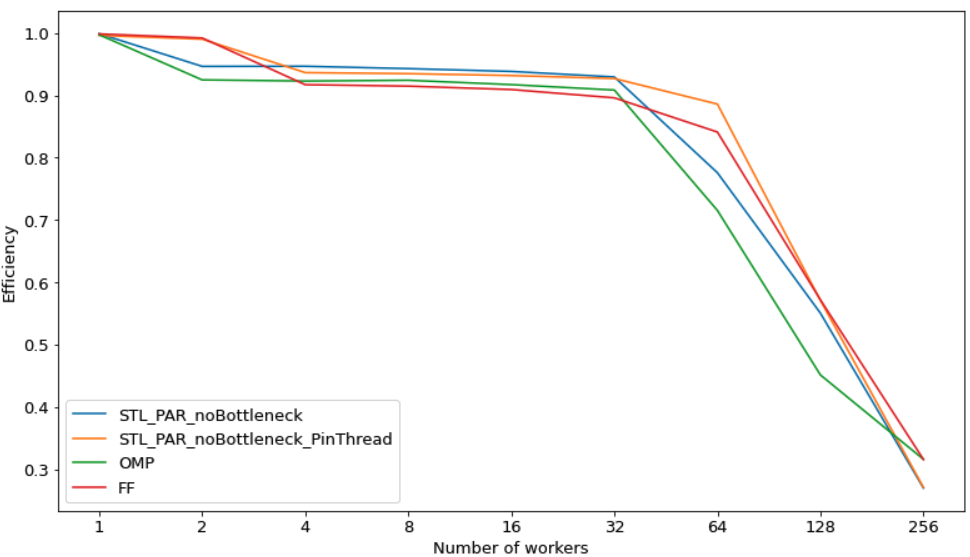
\includegraphics[width=\textwidth]{images/optimized-efficiency.png}
         \caption{Efficiency}
         \label{fig:improved performance}
     \end{subfigure}
        \caption{input 100k s789, K=50}
        \label{fig:three graphs}
\end{figure}

From the plot we can understand that FastFlow and optimized STL C++ parallel implementation showed a better performance in all three measurement. Interestingly, from the plot we can observe that the the movement of the threads from one core to another indeed increases as the number of workers increases; creating an overhead.
\chapter{Conclusion}

In a smaller data-set, openMp seems to be performing better, where as in bigger data-set FastFlow and optimized STL parallel starts to shine. Though getting the ideal result is impossible, I was able to get relatively good performance in all implementations. \\


This project helped me to understand how to analyze and optimize sequential code for much better possible execution time and how to wisely utilize available resources. Even though using pure Standard Template Library gives you much more flexibility in your implementations and design choices, It is amazing to see how the libraries I used provided me similar or better performance with a simple and small lines of codes. Especially, I am surprised by the performance gain and simplicity to use FastFlow.

\section{Future works}
To store k-nearest neighbours, I used a priority queue over a vector with custom compare function which gives us a time complexity of $O(n)$ in insertion and deletion operations. We could improve this complexity by using a heap which will give us a time complexity of $O(logn)$ in insertion and deletion operation and $O(1)$ in finding max and min which could be a better improvement if we were to use bigger $k-value$. I left this change for future improvements. \\

It is also possible to remove the square root found in the formula to calculate euclidean distance. We could save additional computation time without changing the final result.

\section{Folder structure and how to build project}
In the file attached along with this report, all implementation files and necessary scripts to successfully run the program will be found. The file contains 6 folders.

\begin{itemize}
  \item \verb|\bin| folder contains all the executable files.
  \item \verb|\data| folder contains the three data-set used for testing the different implementations.
  \item \verb|\fastflow| is where the FastFlow library is cloned.
  \item \verb|\outputs| folder contains the output of each algorithms or implementations. Each line contain a point id and list of space separated $k$ points closest to the point.
  \item \verb|\src| folder contains utimer class for measure running time of the algorithms and utility functions and data structures used in the program.
  \item \verb|\Test-result| folder contains test result data and visualization of the plots.
\end{itemize}

To build the project issue the \verb|make all| or just \verb|make| command from inside the folder \verb|\Multi-Thread-KNN|. This command will generate the executables inside \verb|bin| folder. Running each executable with no parameter will provide the correct parameters and their orders. Each executable have \verb|-d| optional flag which basically ignores writing the result to the file.\\

To run a single script, the following issue can be issued from inside the project folder. Important thing is that, \verb|/bin/stl_seq_knn| only has two important parameter, \verb|k-value| and \verb|test-data|.

\begin{minted}{bash}
#!/bin/bash
$ ./bin/stl_seq_knn 50 data/input_50k_s456.txt -d           #optional -d
\end{minted}

For the other implementations, there is \verb|nw|, number of workers important parameter. In the following command \verb|nw| is provided as 256. 

\begin{minted}{bash}
#!/bin/bash
$ ./bin/stl_par_knn 256 50 data/input_50k_s456.txt -d      #optional -d
\end{minted}

Additionally, one bash script called \verb|executeTest.sh| is provided to aid the testing of the implementations. The parameter for this script are \verb|k-value| and \verb|runs|. Running time of each algorithm will be averaged over the number of \verb|runs|.

\begin{minted}{bash}
#!/bin/bash
$ ./executeTest.sh 50 3    # k-value = 50 and runs=3
\end{minted}

To generate test data \verb|/bins/generate2d| executable can be used. The parameters are \verb|start|, \verb|end|, \verb|seed|, \verb|amount| and \verb|file name| respectively. For \verb|file name| you don't need to specify file extension. The following command will generated 1000 2d points, each coordinate value between -100 and 100 with 123 seed value. File will be automatically stored in \verb|data/input_1k_points.txt| 

\begin{minted}{bash}
#!/bin/bash
$ ./bin/generate2d -100 100 123 1000 input_1k_points
\end{minted}

\begin{thebibliography}{9}
\bibitem{a} M. Danelutto, DISTRIBUTED SYSTEMS: PARADIGMS AND MODELS, 2014.
\bibitem{a} Structured Parallel Programming: Patterns for Efficient Computation - Michael McCool, James Reinders and Arch D. Robison.
\bibitem{a} https://www.openmp.org/wp-content/uploads/omp-hands-on-SC08.pdf

\end{thebibliography}
\newpage

\appendix

\begin{figure}
     \centering
     \begin{subfigure}[b]{0.45\textwidth}
         \centering
         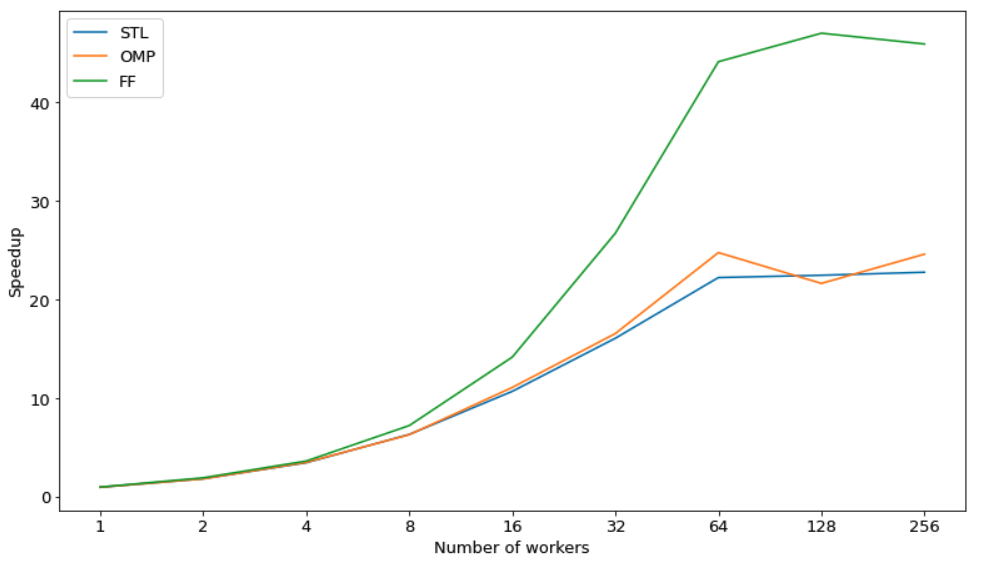
\includegraphics[width=\textwidth]{images/main-20k/speedup.png}
         \caption{Speed up}
         \label{fig:y equals x}
     \end{subfigure}
     \hfill
     \begin{subfigure}[b]{0.45\textwidth}
         \centering
         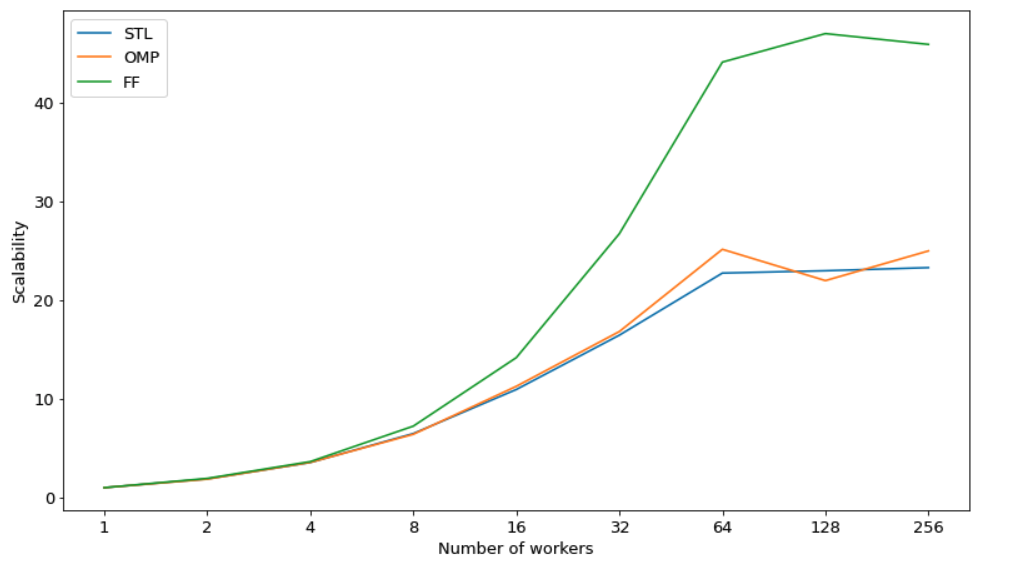
\includegraphics[width=\textwidth]{images/main-20k/scalability.png}
         \caption{Scalability}
         \label{fig:three sin x}
     \end{subfigure}
     \hfill
     \begin{subfigure}[b]{0.45\textwidth}
         \centering
         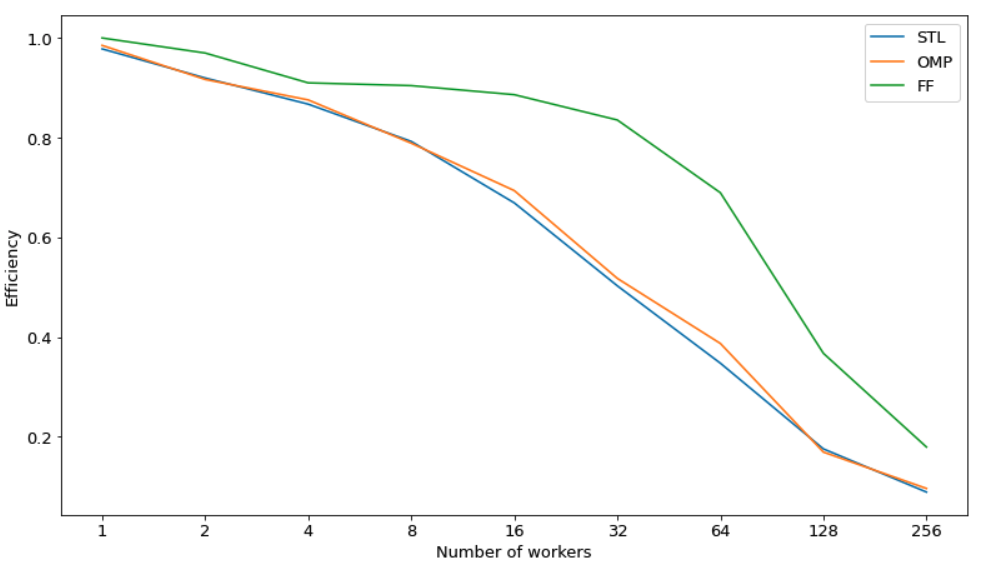
\includegraphics[width=\textwidth]{images/main-20k/efficiency.png}
         \caption{Efficiency}
         \label{fig:improved performance}
     \end{subfigure}
        \caption{input\_20k\_s123.txt, K=50, with no performance improvement}
        \label{fig:three graphs}
\end{figure}
\begin{figure}
     \centering
     \begin{subfigure}[b]{0.45\textwidth}
         \centering
         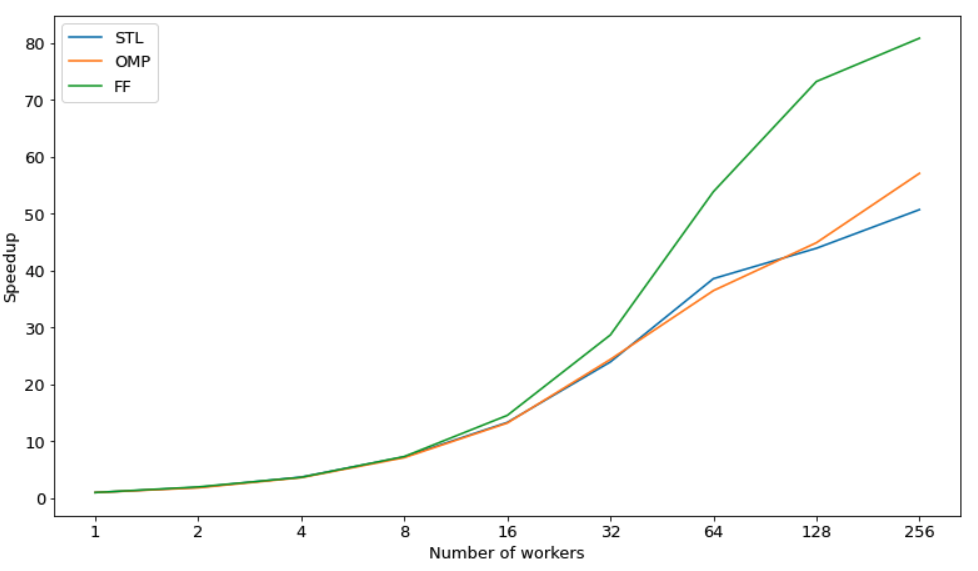
\includegraphics[width=\textwidth]{images/main-50k/speedup.png}
         \caption{Speed up}
         \label{fig:y equals x}
     \end{subfigure}
     \hfill
     \begin{subfigure}[b]{0.45\textwidth}
         \centering
         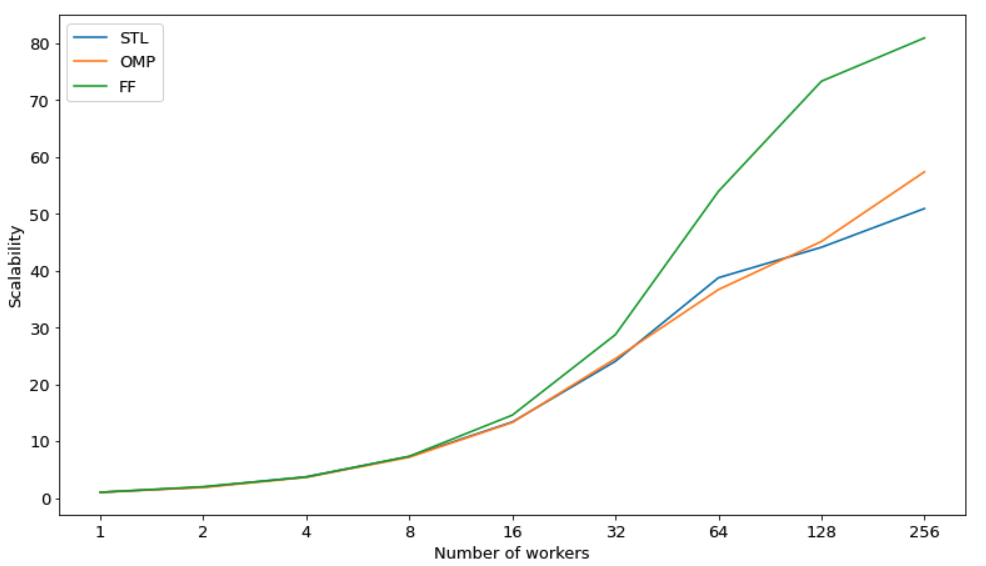
\includegraphics[width=\textwidth]{images/main-50k/scalability.png}
         \caption{Scalability}
         \label{fig:three sin x}
     \end{subfigure}
     \hfill
     \begin{subfigure}[b]{0.45\textwidth}
         \centering
         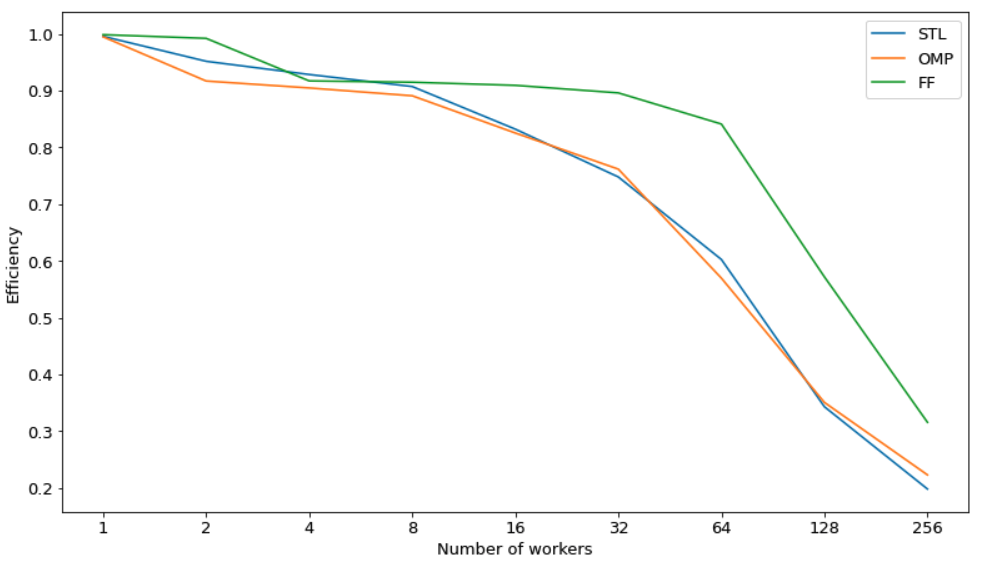
\includegraphics[width=\textwidth]{images/main-50k/efficiency.png}
         \caption{Efficiency}
         \label{fig:improved performance}
     \end{subfigure}
        \caption{i{input\_50k\_s456.txt, K=50, with no performance improvement}}
        \label{fig:three graphs}
\end{figure}

\begin{figure}
     \centering
     \begin{subfigure}[b]{0.45\textwidth}
         \centering
         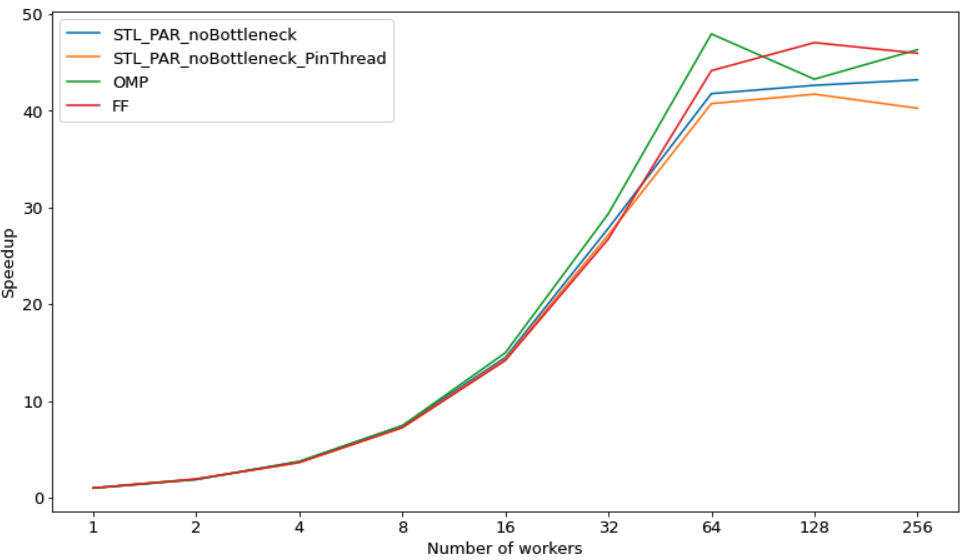
\includegraphics[width=\textwidth]{images/optimized-20k/speedup.png}
         \caption{Speed up}
         \label{fig:y equals x}
     \end{subfigure}
     \hfill
     \begin{subfigure}[b]{0.45\textwidth}
         \centering
         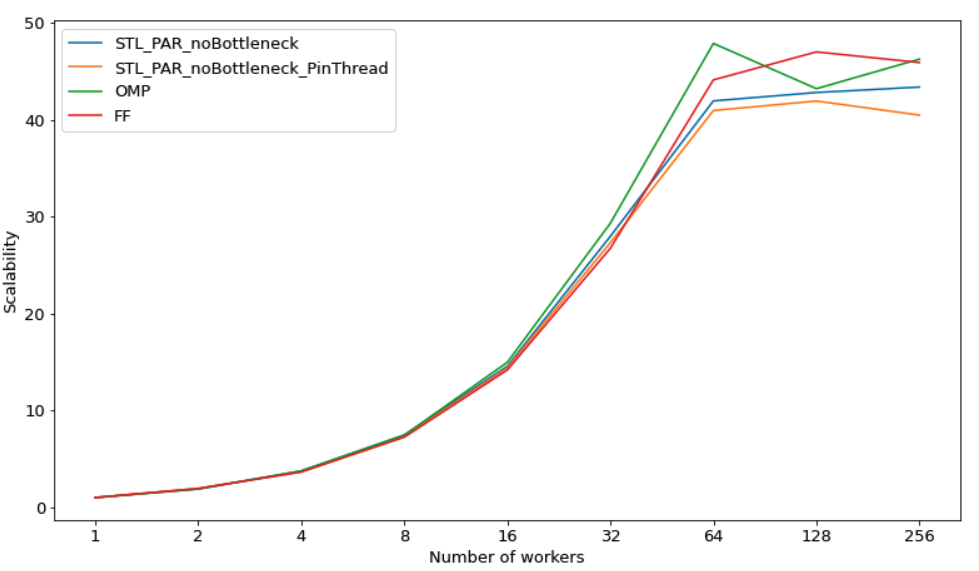
\includegraphics[width=\textwidth]{images/optimized-20k/scalability.png}
         \caption{Scalability}
         \label{fig:three sin x}
     \end{subfigure}
     \hfill
     \begin{subfigure}[b]{0.45\textwidth}
         \centering
         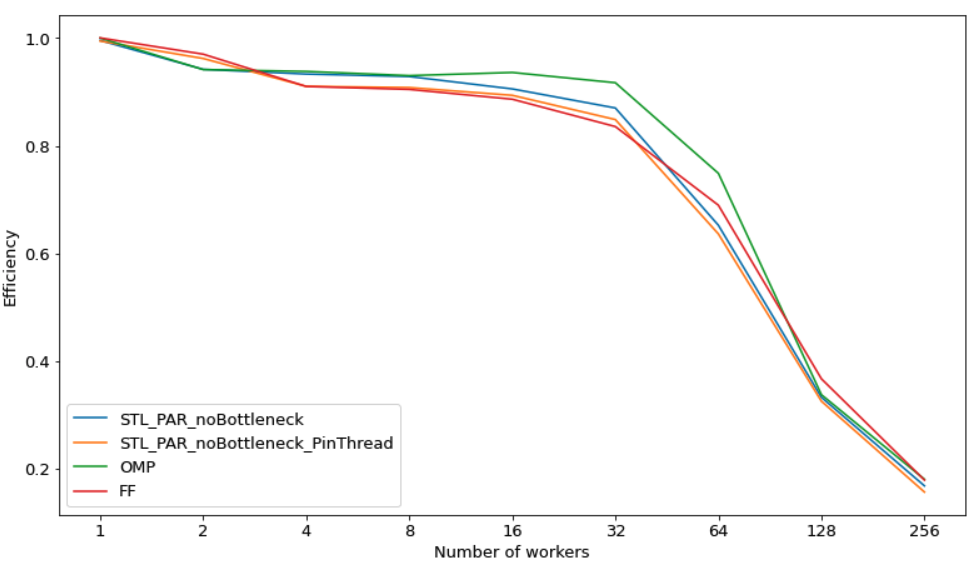
\includegraphics[width=\textwidth]{images/optimized-20k/efficiency.png}
         \caption{Efficiency}
         \label{fig:improved performance}
     \end{subfigure}
        \caption{{input\_20k\_s123.txt, K=50, with performance improvement}}
        \label{fig:three graphs}
\end{figure}
\begin{figure}
     \centering
     \begin{subfigure}[b]{0.45\textwidth}
         \centering
         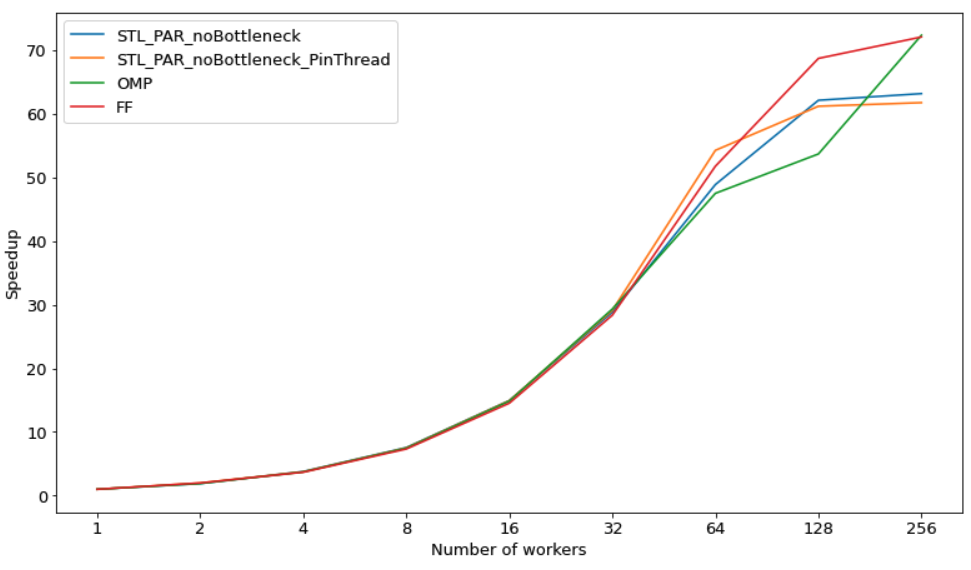
\includegraphics[width=\textwidth]{images/optimized-50k/speedup.png}
         \caption{Speed up}
         \label{fig:y equals x}
     \end{subfigure}
     \hfill
     \begin{subfigure}[b]{0.45\textwidth}
         \centering
         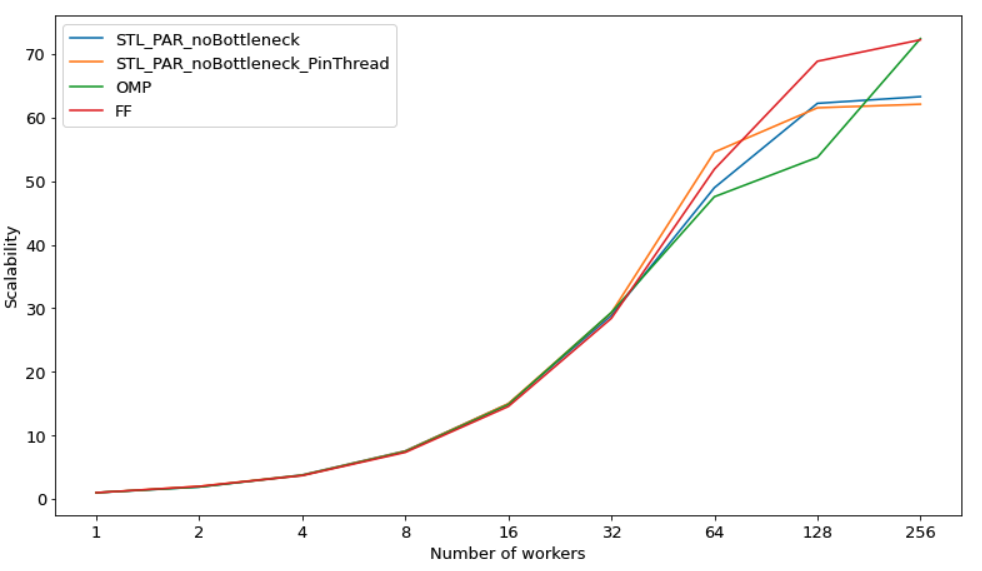
\includegraphics[width=\textwidth]{images/optimized-50k/scalability.png}
         \caption{Scalability}
         \label{fig:three sin x}
     \end{subfigure}
     \hfill
     \begin{subfigure}[b]{0.45\textwidth}
         \centering
         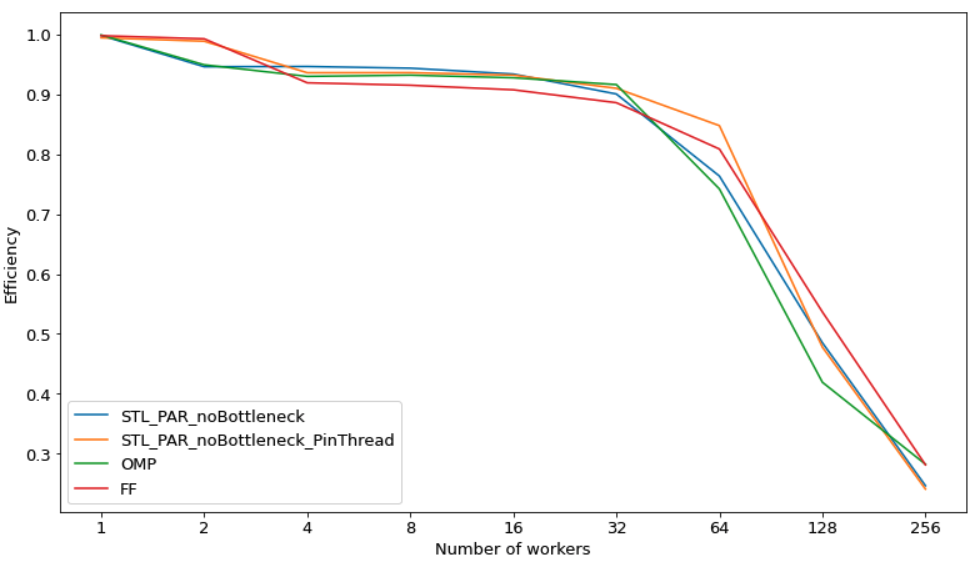
\includegraphics[width=\textwidth]{images/optimized-50k/efficiency.png}
         \caption{Efficiency}
         \label{fig:improved performance}
     \end{subfigure}
        \caption{{input\_50k\_s456.txt, K=50, with performance improvement}}
        \label{fig:three graphs}
\end{figure}

\end{document}
